    %%%%%%%%%%%%%%%%%%%% CHAPTER  %%%%%%%%%%%%%%%%%%%%%%%
    %------------------------------------- Preeliminares-------
    \chapter{Preliminares}
    Antes de poder hablar del Aprendizaje profundo, o de Redes Neuronales Convolucionales, es importante sentar las bases matemáticas y computacionales requeridas para su estudio. A continuación, se presentan algunas definiciones y resultados conocidos de temas tales como cálculo, álgebra y ciencias de la computación.
    \section{Resultados de Cálculo y Álgebra lineal}
    \begin{definition}[Polinomio de Taylor]
        Sea $f$ una función $n$ veces diferenciable, y sean $$a_k = \frac{f^{(k)}(a)}{k!}.$$
        Definimos el Polinomio de Taylor de grado $n$ para $f$ en $a$ como
        $$P_{n,a}(x) = a_0 + a_1(x-a) + \cdots + a_n(x-a)^n.$$
    \end{definition}
    El polinomio $P_{n,a}(x)$ ha sido definido de manera que $P_{n,a}(a) = f^{(k)}(a)$ para $0\leq k \leq n$.
    \begin{definition}
        Sea $f$ una función tal que $P_{n,a}(x)$ existe, definimos el término  residual $R_{n,a}(x)$ como 
        \begin{equation}
            R_{n,a}(x) = f(x) - P_{n,a}(x).
        \end{equation} 
    \end{definition}
    \begin{theorem}[Teorema de Taylor]
        Supóngase que $f^{(1)}$, $f^{(2)}$, ..., $f^{(n+1)}$ están definidos en $[a,x]$. Entonces 
        \begin{equation}
            R_{n,a}(x) = \frac{f^{n+1}(t)}{(n+1)!}(x-a)^{n+1}
        \end{equation}
        para algún $t\in (a,x)$.
    \end{theorem}

    \begin{definition}
        Sea $x$ una característica en $\mathbb R^{h\times w\times d}$. La vectorización de $x$, denotada $X = \text{vec}(x)$ es un vector en $\mathbb R^{hwd}$ tal que 
        \begin{equation}
            X_{(k-1)hw + (i-1)w + j} = x_{i,j,k},
        \end{equation}
        para todos $i=1,2, ..., h$, $j = 1, 2, ..., w$, $k= 1,2,..., d$.
    \end{definition}
    \textcolor{red}{explicar que es una característica (feature). Además, en la definición de convolución uso una imagen $I$, tal vez sea más consistente escribir una característica $x$.}
    \begin{definition}
        Una matriz $H$ es llamada \textsl{Circulante} si es de la forma
        \begin{equation}
            H = \begin{bmatrix}
                h_0 & h_1 & \cdots & h_{N-1} \\
                h_{N-1} & h_0 & \cdots & h_{N-2} \\
                \vdots & \vdots &  & \vdots \\
                h_1 & h_2 & \cdots & h_{0} \\
            \end{bmatrix}
        \end{equation}
        ya que $H$ queda completamente determinada con la primera fila, es posible escribir $H = \text{circ}(h_0, ..., h_{N-1})$.
    \end{definition} 
    \begin{definition}
        \label{doubly_circulant_matrix}
        Una matriz $H$ es llamada \textsl{Doblemente Circulante por Bloques} si es de la forma
        \begin{equation}
            H = \begin{bmatrix}
                H_0 & H_1 & \cdots & H_{N-1} \\
                H_{N-1} & H_0 & \cdots & H_{N-2} \\
                \vdots & \vdots &  & \vdots \\
                H_1 & H_2 & \cdots & H_{0} \\
            \end{bmatrix} = \text{circ}(H_0, ..., H_{N-1})
        \end{equation}
        dónde $H_i = \text{circ}(h_{i,0}, ..., h_{i, N-1})$.
    \end{definition}
    \begin{definition}
        Sean $A$ y $B$ dos conjunto. El producto cartesiano $A \times B$ se define como
        \begin{eqnarray}
            A \times B &= \{(a,b) : a\in A \text{ y } b\in B\}.
        \end{eqnarray}
        De igual manera sean $A_1, ..., A_s$ son conjuntos, el producto cartesiano se define como
        \begin{equation}
            A_1\times A_2 \times ... \times A_s = \{(a_1,..., a_s): a_i\in A_i, \quad i= 1,...,s\}.
        \end{equation}
        De modo natural, se define $A^n :=  A \times A \times ... \times A$ donde $A$ se repite $n$ veces.
    \end{definition}
    A su vez, nos es conveniente destacar otra notación
    
    \begin{notation}
        Sean $a_1, ..., a_n\in \mathbb N$. Definimos $\mathbb R^{a_1 \times a_2 \times ... \times a_s} := \mathbb R^{a_1} \times ... \times \mathbb R^{a_s}$
    \end{notation}

    \begin{definition}
        Sean $u,v\in \mathbb R^n$, el producto punto de $u$ con $v$ denotado como $u\cdot v$ es
        \begin{equation}
            u_1v_1 + u_2+v_2 + ... + u_nv_n
        \end{equation}
        donde $u_i$ y $v_i$ representan la $i$-ésima entrada de los vectores $u$ y $v$ respectivamente.
    \end{definition}

    \begin{definition}
        Una función vectorial es una función de la forma $f:\mathbb R \to \mathbb R^n$.
    \end{definition}

    \begin{definition}
        La derivada $f'$ de una función vectorial $f: \mathbb R \to \mathbb R^n$ se define como
        \begin{equation}
            f'(t) = \lim_{h\to 0} \frac{f(t+h)- f(t)}{h\to 0}.
        \end{equation}
    \end{definition}
    Sin embargo, en la práctica, no es necesario utilizar la definición, pues 
    \begin{theorem}
        La derivada $f'$ de una función vectorial $f = (f_1, f_2, ..., f_n)$, con $f_i: \mathbb R \to \mathbb R$ es
        \begin{equation}
            f'(t) = (f_1'(t), f_2'(t), ..., f_n'(t)).
        \end{equation}
    \end{theorem}
    \begin{definition}[Gradiente]
        Sea $f: \mathbb R^n \to \mathbb R$. El gradiente de $f$ es el vector conformado por las derivadas parciales en cada una de las $n$ variables:
        \begin{equation}
            \nabla f = \left(\frac{\partial f}{\partial x_1}, ..., \frac{\partial f}{\partial x_n}\right).
        \end{equation}
    \end{definition}
    \begin{proposition}[Regla de la cadena]
        Sea $f: \mathbb R^n \to \mathbb R$ y $v: \mathbb R \to R^n$. Es posible hallar la derivada de la composición.
        \begin{equation}
            \frac{d}{dt}(f\circ g) = \nabla f \cdot  v'(t)
        \end{equation}
    \end{proposition}

    \begin{definition}[Notación O-grande (Big O)]
        Sean $f$ y $g$ funciones $f,g:\mathbb N \to \mathbb R^+$. Decimos que $f(n) = \mathcal O(g(n))$ si existen enteros positivos $c$ y $n_0$ tales que para cualquier entero $n\geq n_0$,
        \begin{equation}
            f(n) \leq cg(n).
        \end{equation}
        Cuando $f(n) = \mathcal O(n)$, decimos que $g(n)$ es una cota asintótica superior de $f(n)$,
    \end{definition}

    %------------------------------------- Vision computacional -------
    \section{Visión Computacional}
    El problema de clasificación de imágenes, pertenece a la rama de la visión computacional. La siguiente definición de imagen fue extraída del libro \cite{computer_vision}.
    \begin{definition}
        Una \textsl{imagen digital} es una función $I:  D \subset \mathbb Z^2 \to U$. Dónde el domino es un rectángulo con coordenadas enteras $D = [1,M]\cap \mathbb Z \times [1,N] \cap \mathbb Z$. La terna $(x,y,u)$ se conoce como pixel.
        \begin{itemize}
            \item Cuando las imágenes son a escala de grises se tiene que $U=[0,255]\cap \mathbb Z$. Es decir que $u\in U$ es un valor de 0 a 255.
            \item Si las imágenes son a color, consideramos $U=([0,255]\cap \mathbb Z)^3$. Es decir que $u\in U$ es una terna de valores de 0 a 255. A cada entrada de la terna se conoce como un canal de color.
        \end{itemize}
    \end{definition}
    Es posible representar una \textsl{imagen digital} $I$ como un \textsl{Tensor}, de la siguiente manera.
    \begin{equation}
        T_{i,j,k} = u_k, \quad u = I(i,j)
    \end{equation}

    \textcolor{red}{Definir en algún punto lo que es un tensor}
    %------------------------------------- Inteligencia artificial y aprendizaje profundo -------    
    \section{Inteligencia artificial y Aprendizaje profundo}
    El \textsl{Aprendizaje de Máquina} es un caso particular de la inteligencia artificial, en donde la máquina aprende de los datos proporcionados. Para entender este concepto es importante definir qué significa aprender \cite{Mitchell}.
    \begin{definition}
        Se dice que un programa de computadora aprende de la experiencia $E$ respecto a un conjunto de tareas $T$ y medida de rendiminto $P$ si el rendimiento en las tareas en $T$, medido con $P$ mejora gracias a la experiencia $E$.
    \end{definition}
    Ya que aprender, implica mejorar el rendimiento en una tarea específica, sería bueno remarcar algunas de las tareas más comunes en el campo del aprendizaje automático.
    \begin{enumerate}
        \item \textbf{Clasificación.} Consiste en que el modelo reconozca que elementos pertenecen a ciertas clases, teniendo en cuenta sus características. Por ejemplo, distinguir perros de gatos, o en el caso de este proyecto podría ser diferenciar entre polen y polvo
        \item \textbf{Regresión.} Aquí lo que se busca es usar la información existente para tener una predicción aproximada de algún escalar. Por ejemplo, predecir el precio de una casa, dadas sus características (ubicación, número de cuartos, antiguedad, etc).
        \item \textbf{Agrupamiento (Clustering).} Este es un méto de aprendizaje no supervisado, que tiene como objetivo detectar similitudes entre las instancias, y separarlas en grupos de elementos similares entre sí.
    \end{enumerate}
    
     %------------------------------------- Overfitting y Underfitting -------    
    \subsection{Sobreajusto y Desajuste}
    En el aprendizaje automático, nuestro modelo aprende de un conjunto de entrenamiento $\mathcal X$. Sin embargo, una vez que nuestro modelo ha aprendido ¿Cómo podemos determinar que aprendió correctamente o que desempeñó de manera satisfactoria su tarea? La manera de determinar que nuestro modelo es bueno, es probando su capacidad de hacer predicciones con datos que no haya utilizado durante el entrenamiento. Para ello, es necesario un conjunto de imágenes nuevas $\mathcal X'$ al cual llamaremos conjunto de prueba. 

    El proceso de entrenamiento consiste en optimizar una función en nuestro conjunto $\mathcal X$, donde es posible encontrar una medida de error, la cual se conoce como \textsl{error de entrenamiento}. Sin embargo, nuestro objetivo es reducir el error en nunestro conjunto de prueba, el cuál se denomina \textsl{error de prueba}. El desempeño correcto de un modelo en el conjunto de prueba se conoce como \textsl{generalización} y por ello el error de entrenamiento también es conocido como \textsl{error de generalización}

    Asumimos que los elementos en nuestros conjuntos de datos son \textsl{independientes} y además que el conjunto de entrenamiento y el de prueba están \textsl{identicamente distribuidos}, lo cual se conoce como las suposiciones IID. Con estas suposiciones y debido a la naturaleza del entrenamiento, se espera que el error de prueba se reduzca a la par que el error de entrenamiento, y lo más normal es que el error de prueba sea mayor que el de entrenamiento.

    Sin embargo, el conjunto de funciones que puede adoptar un modelo, depende de la cantidad de parámetros que este tenga, lo cual se conoce como \textsl{capacidad}. Con una capacidad suficiente, siempre es posible hacer un mapeo perfecto entre entradas y etiquetas. Sin embargo, no es la función que se adapte mejor a los datos de entrenamiento la que es más conveniente, sino la que generalice mejor. Cuando la diferencia entre el error de entrenamiento y el error de generalización se acrescenta se dice que el modelo sufre de un \textsl{sobreajuste}. Cuando la capacidad de un modelo es muy reducida, puede ocurrir que no sea posible reducir el error de entrenamiento con lo que el modelo sufre de un \textsl{desajuste}.
    % imagen de sobreajuste y desajuste. 

    \subsection{Regularización}
    Cuando se entrena un modelo, son necesarias dos partes: 
    \begin{enumerate}
        \item Optimización: En donde, se busca minimizar la función de costo.
        \item Generalización: Es importante que las predicciones de nuestro modelo sean aplicables con datos que no hayan sido vistos en el entrenamiento.
    \end{enumerate}
    Sin embargo, no es fácil conseguir ambos objetivos simultáneamente. En vez de priorizar alguno de los dos, la \textsl{regularización} pretende lograr que se satisfagan ambos de la mejor manera. Es decir, \textsl{la regularización es cualquier modificación en el algoritmo de entrenamiento, cuyo objetivo sea reducir el error de generalización, pero no el error de entrenamiento}.
    % \begin{example}(Weight Decay)
        
    % \end{example}
    % \begin{figure}[H]
    %     \includegraphics{regularization.png}
    % \end{figure}
    \textcolor{red}{Insertar imágenes con ejemplos}
    Una de las formas más comunes de regularizar un modelo que aprende la función $f(x, \theta)$, es agregando una penalización $R(\theta)$ a la función de costo, considerando $\theta$ como los parámetros.
    \subsection{Función de activación.
    }
    Con la intención de ampliar el conjunto de funciones que un modelo puede predecir, en cada capa de nuestras redes neuronales, se compone una función no lineal denominada \textsl{función de activación}. En caso de no incluirla, el conjunto de funciones disponibles para nuestro modelo serían sólo funciones lineales, debido a que la composición de dos funciones lineales $L_1$ y $L_2$ da lugar a otra función lineal $L_1 \circ L_2$.

    Existen muchos ejemplos de funciones no lineales. En un principio se usaban funciones suaves como la función \textsl{sigmoidal} $(1+\exp(x))^{-1}$, la tangente hiperbólica $\tanh(x)$, o la función \textsl{Softplus} $\dfrac{1}{\beta} \log(1+ \exp(\beta x))$. Sin embargo, las tendencias modernas prefieren las funciones no suaves como es el caso de la más popular \textsl{ReLU} $\max(x,0)$.

    \begin{figure}[H]
        \centering
        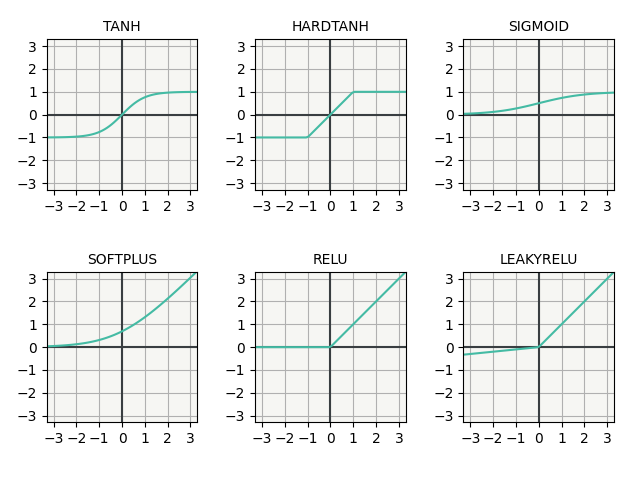
\includegraphics[width=6in]{../cap1_preliminares/src/activations.png}
        \caption{\textcolor{red}{Usar una imagen propia}}
    \end{figure}
    
    % Transferemcia de aprendizaje
    \subsection{Transferencia de aprendizaje}
    La transferencia de aprendizaje en el campo del aprendizaje profundo, es un concepto motivado por la psicología, que se basa en usar conocimientos adquiridos para cierta tarea $A$, con el objetivo de aprender alguna tarea $B$. Por ejemplo, si una persona sabe bailar salsa, posiblemente pueda usar esos conocimientos para aprender a bailar bachata. 

    En la mayoría de los casos, los conjuntos de datos tienen una cantidad limitada de imágenes etiquetadas. Una posible solución a este problema, es usar \textsl{aprendizaje semisupervisado}, el cuál requiere algunas imágenes etiquetadas, pero también se pueden usar varias imágenes no etiquetadas. Sin embargo, incluso los conjuntos de datos no etiquetados, pueden ser insuficientes. Cuando se tienen conjuntos de datos muy pequeños, es posible apoyarse de modelos pre-entrenados con millones de imágenes, con la esperanza de que las características aprendidas anteriormente, sean de utilidad en el nuevo conjunto de datos.
    % Conjuntos desbalanceados
    \subsection{Conjuntos desbalanceados}
    Cuando se enfrenta el problema de clasificación, digamos con $m$ clases, uno esperaría que tengamos suficientes ejemplos de cada clase. Más aún, para que nuestro modelo no tenga ningún sesgo por ninguna clase, es preferible que en nuestro conjunto de entrenamiento, todas las clases tengan una cantidad similar de ejemplos. De lo contrario, nuestro modelo podría ser entrenado con demasiados elementos de una clase particular $mathcal C$, y tendería a clasificar muchos elementos en la clase $\mathcal C$. Además de esto, si nuestro conjunto de prueba también está desbalanceado, no se vería reflejado el sesgo en métricas comunes como la exactitud y la precisión.

    \begin{definition}
    \label{balanced}
        Sea $\mathcal C$ un conjunto de datos, cuyas clases son $\mathcal C_1, ..., \mathcal C_m$. Un conjunto de datos se dice balanceado con tolerancia de $\epsilon$ si 
        \begin{equation}
            1-\epsilon \leq \frac{|C_i|}{|C_j|} \leq 1 + \epsilon, \quad i,j = 1,2, ..., m.
        \end{equation}
        Un conjunto es desbalanceado bajo la tolerancia $\epsilon$ si no es balanceado.
    \end{definition}
    Para efectos prácticos, diremos que un conjunto balanceado con tolerancia $\epsilon = 0.1$
    \begin{example}
        Supóngase ahora que dada una lista de características, se quisiese clasificar a las personas infectadas de COVID-19. En México el índice de positividad es del $17\%$ \cite{}. Por lo que si se toman todas las pruebas realizadas tendríamos la siguiente razón:
        \begin{equation}
            \frac{|C_{Neg}|}{|C_{Pos}|} = 4.8823 > 1.1.
        \end{equation}
        El tamaño de la clase de pruebas negativas es casi 5 veces mayor al tamaño de la clase de pruebas positivas. Por consiguiente, estaríamos en presencia de un conjunto de datos desbalanceado.
    \end{example}
    \begin{figure}[H]
        \centering
        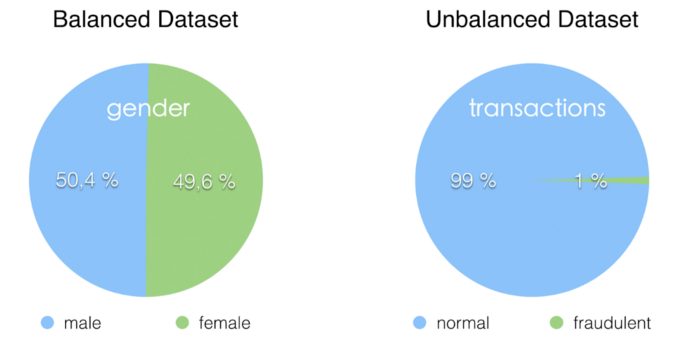
\includegraphics[width=6in]{../cap1_preliminares/src/unbalanced.png}
        \caption{\textcolor{red}{Usar una imagen propia}}
    \end{figure}
    \subsubsection{Afrontar un problema con un conjunto desbalanceado}
    La forma principal de lidiar con un conjunto desbalanceado es, valga la redundancia \textsl{balancear el conjunto}. Es decir, forzar al datset a tener clases cuyos tamaños coincidan. Para conseguir esto, es posible seguir distintas estrategias.
    \begin{itemize}
        \item \textbf{Submuestreo.} Consiste en tomar la classe \textcolor{red}{mayoritaria} (La clase con menor número de elementos) y eliminar algunas instancias, de modo que el conjunto quede balanceado. La manera más sencilla, es tomando elementos aleatorios del conjunto. Sin embargo, esto puede retirar instancias que contengan información esencial, por lo que sólo es recomendable en caso de tener un conjunto de datos muy grande.

        Otros algoritmos, heurísticos se basan en dos diferentes modelos de teoría de ruido. Algunos investigadores consideran que las instancias cercanas a los márgenes de clasificación de dos clases, son consideradas ruido. Por otro lado, algunos investigadores consideran que las instancias presentes en vecindades de varias etiquetas distintas, se pueden considerar como ruido. De modo que en lugar de remover elementos aleatorios, estas estrategias implican hacer el submuestreo tomando en cuenta únicamente las instancias que no sean ruido.

        \item \textbf{Sobremuestreo.} Al igual que en el submuestreo, existe el sobremuestreo aleatorio, el cual se basa en crear copias idénticas de las instancias de la clase minoritaria, de modo que la nuestra clase minoritaria alcance la magnitud del resto de clases. Al aplicar este método, se incrementa el riesgo de sobreajustar el modelo. 

        Otras algoritmos de sobremuestreo, generan instancias sintéticas para incremantar la cantidad de datos en una clase. Existen diversas formas de conseguir esto. Una posibilidad, es usando el aumento de datos únicamente en la clase minoritaria, permitiendo rotaciones, traslaciones y otras transformaciones. Existe también algoritmos como el VAE, SMOTE, MSMOTE. 

    \end{itemize}

    \begin{figure}[H]
        \centering
        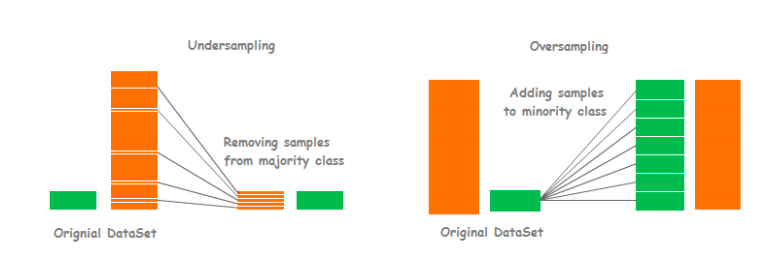
\includegraphics[width=6in]{../cap1_preliminares/src/undersampling_oversampling.png}
        \caption{\textcolor{red}{Usar una imagen propia}}
    \end{figure}

    \subsubsection{Métricas distintas a la exactitud}
    Como hemos mencionado antes, la exactitud no debe ser la única métrica a considerar en un problema con conjunto de datos desbalanceado. La razón es simple: es posible obtener una muy buena exactitud sin realmente hacer predicciones de nuestra clase minoritaria.
    \begin{example}
        \label{diff_metrics}
        Si tenemos un conjunto de datos con dos clases, tal que una clase $C_1$ representa el $99\%$ de las instancias, y la clase $C_2$ el $1\%$ restante. Si tomamos el clasificador $f: \mathcal C \to \{1,2\}$, $f(x) = 1$. Claramente nuestra exactitud sería del $99\%$, pero las predicciones de nuestra clase minoritaria aciertan un $0\%$ de las veces.
    \end{example}{}
    Una forma de sobrellevar el efecto visto en el ejemplo \ref{diff_metrics} es analizando el desempeño del clasificador para cada clase por separado y luego hacer un promedio. En el caso de nuestro ejemplo todas las instancias que en verdad pertenecen a la clase 1, fueron clasificadas correctamente (1.0), y las instancias que pertenecen a la clase 2, fueron clasificadas todas incorrectamente (0.0). Con lo con esta nueva métrica tendríamos una puntuación de $\frac{1.0 + 0.0}{2} = 0.5$. En el capítulo \ref{experimentos} se definen formalmente las métricas relevantes para este trabajo. Sin embargo, las métricas más utilizadas para este tipo de problemas son las siguientes:
    \begin{itemize}
        \item Confussion matrix: De ésta matriz, se pueden obtener métricas útiles tales como Specificity, Sensitivity, Precision, Recall
        \item F1-score: La media armónica de precision y recall
        \item ROC curves
        \item Logloss
        \item Kappa: Exactitud de la clasificación, normalizada por el desbalance de clases en nuestros datos.
    \end{itemize}

    % Perceptrón {}{}
    \subsection{Redes completamente conectadas}

    \subsection{Clasificación de imágenes}
    Para poder clasificar las imágenes, los algoritmos de inteligencia artificial extraen características importantes de una imagen. ¿Qué puede ser tomado en cuenta como importante? Podría pensarse que las esquinas, los bordes u otros detalles. Sin embargo, los algoritmos de aprenizaje automático suelen ser cajas negras, dónde las caraceterísticas relevantes de una imagen, a simple vista no parezcanr
    \begin{definition}[Característica]
        Una característica $x$ es un elemento de $\mathbb R^{w\times h\times d}$, dónde $w,h\in \mathbb N$ representan las dimensiones espaciales y $d$ la cantidad de canales.
    \end{definition}

    \section{Notas del capítulo}
    \begin{enumerate}
        \item  Añadir la referencia: A Comprehensive Survey on Transfer Learning
        \item Falta terminar la sección de transferencia de aprendizaje
        \item Uso términos como exactitud y precisión, cuándo estos se definen en la última sección.
        \item Añadir la referencia de la población de Hombres y Mujeres en el ejemplo 1 de conjuntos desbalanceados
        \item Añadir referencia de positividad de Covid en México en el ejepmlo 2 de conjuntos desbalanceados.
    \end{enumerate}